\section{\'Eclat des lampes}

Les lampes du circuit suivant sont toutes identiques. l'ampèremètre indique une intensité $I = \num{0.60} A.$

\begin{center}
	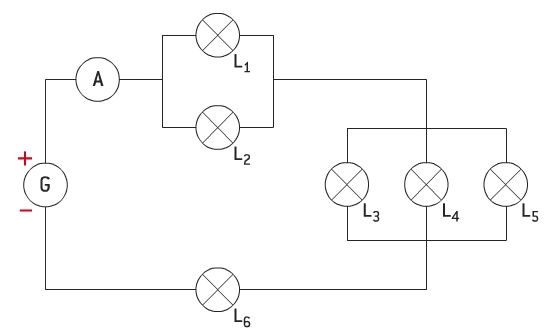
\includegraphics[scale=0.6]{img/ex_16}
\end{center}

\begin{questions}
	\question Quelle sera l'intensité du courant du courant circulant dans chaque lampe ?
	\fillwithdottedlines{3cm}
	
	\question Les lampes vont-elles briller de la même façon ?
	\fillwithdottedlines{2cm}
	
	\question Classer les lampes de celles qui ont l'éclat le plus fort à celles qui ont l'éclat le plus faible.
	\fillwithdottedlines{2cm}
	
\end{questions}